\chapter{معماری نمونه مطالعاتی برنامه پارکینگ}

\section{زمینه برنامه‌ پارکینگ}
هدف از برنامه برقراری ارتباط کاربران با پارکنیگ‌‌های مختلف و فضا‌های خالی در هر پارکینگ است؛ کاربران در این برنامه ها باید بتوانند از مکان‌های خالی در پارکینگ‌های سطح شهر آگاه شوند و امکان رزرو مکان‌های خالی را داشته باشند.در این برنامه تعداد زیاد پارکینگ‌ها در سطح شهر و تغییرات زیاد در وضعیت پارکینگ‌ها سبب پیچیدگی مدیریت سنسور‌ها می‌شود، در حالی که این پیچیدگی نباید خود را در پایگاه کد و سایر مولفه‌های سیستم نشان دهد.به منظور تفکیک دغدغه‌ها، معماری پیشنهادی برای این برنامه معماری لایه‌ای است.

در معماری لایه‌ای، لایه ها مستقل هستند بنابرین گروهی از تغییرات در یک لایه بر لایه های دیگر تأثیر نمی گذارد. با توجه به این ویژگی هر گونه تغییر در ساختار هر لایه این امکان را به ما می‌دهد تا مستقل از سایر لایه‌‌ها به بررسی تغییرات انجام شده بپردازیم. به عنوان مثال تغییر در پروتکل مورد استفاده در سنسور ها در معماری لایه‌ای صدمه ای به ساختار لایه‌های بالاتر نمی‌زند.
\section{معماری پیشنهادی}
با توجه به زمینه مطرح شده برای برنامه پارکینگ‌های شهری، معماری لایه ای پیشنهادی باید دارای لایه‌های شکل \ref{fig:parking_layer} باشد.
\begin{figure}[h]
\centering
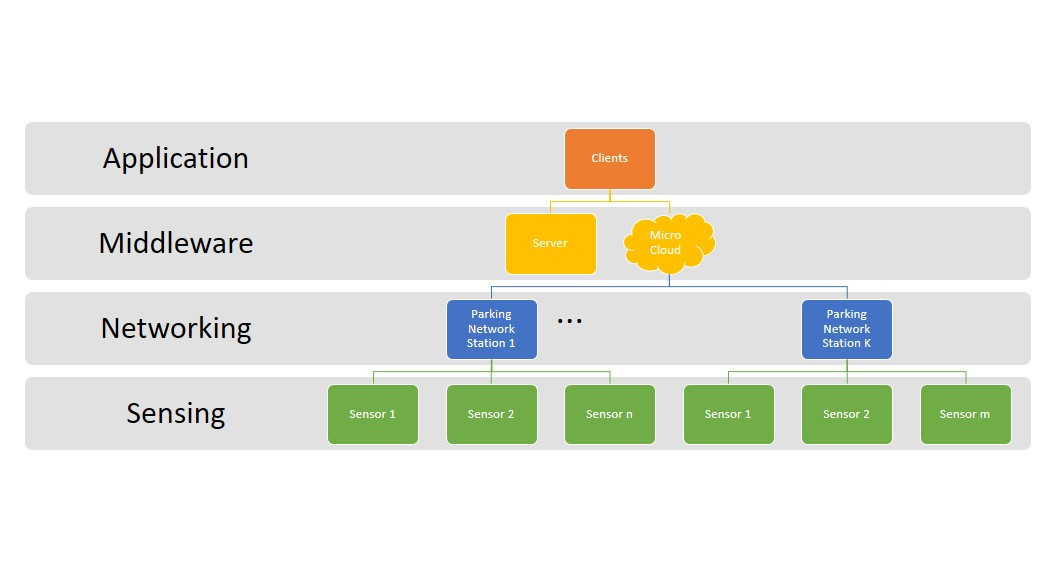
\includegraphics[scale=0.6]{parking_layer.jpg}
\caption{معماری لایه‌ای پیشنهادی برای برنامه پارکینگ‌های شهری}
\label{fig:parking_layer}
\end{figure}
در معماری لایه‌ای پیشنهادی شده حیطه عملکردی هر لایه به شرح زیر است:
\begin{itemize}
\item
لایه‌ی برنامه\LTRfootnote{Application} : برنامه‌های سمت کاربر شامل برنامه‌ی تلفن همراه و نسخه‌های وب در این لایه پیاده سازی می‌شوند و از طریق رابط های از لایه‌ی پایینی خود خدمات را دریافت می‌کنند.
\item
لایه میان‌افزار\LTRfootnote{Middleware} : در این لایه اطلاعات پارکینگ ها به صورت لحظه‌ای دریافت می‌شود و پس از پردازش خدماتی که کاربران در لایه‌ی برنامه نیاز دارند، در اختیارشان قرار داده می‌شود.
\item
لایه شبکه \LTRfootnote{Networking} : لایه‌ی شبکه به منظور ارتباط آسان تر سنسور‌ها با لایه‌ی میان افزار تعبیه شده است. اگر قرار بود هر یک از سنسور‌ها خود مستقلا به لایه‌ی میان‌افزار وصل شوند پیچیدگی شبکه و مدیریت آن بسیار دشوار بود.لایه‌ی شبکه با تجمیع اطلاعات سنسور‌ها ضمن کشف خرابی یا اطلاعات ناصحیح در میان سنسور‌ها با پروتکل‌های مطمئن تری ضمن هزینه کمتر اطلاعات را در اختیار لایه میان‌افزار قرار می‌دهد.
\item
لایه سنسور‌ها\LTRfootnote{Sensing} : سنسور‌ها از نوع های مختلف در این لایه قرار دارند و این لایه با محدود‌سازی پیچیدگی‌های سخت‌افزاری مانع از انتشار آن به لایه‌های بالاتر خواهد شد.
\end{itemize}
\section{نیازمندی‌های پوشش‌داده شده توسط معماری}